\documentclass[12pt,a4paper,norsk]{article}
\usepackage[norsk]{babel}
\usepackage[utf8]{inputenc}
\usepackage{minted}
\usepackage{graphicx}
\usepackage{hyperref}
\title{\vspace{-3cm}Oppgaver til leksjon nr. 23 I nettsikkerhet}
\author{Bjørn Kristian Punsvik}
\date{\today}

\begin{document}
\maketitle
\section*{Oppgave 1}
\subsection*{a) Hva kunne de gjort for å forhindre at dette skjedde?}
Her gjelder preventive tiltak. Etter artikkelen å dømme har de 2 dører mellom utsiden og plassen ingeniørene oppbevarte pc-ene. Første dør ser vi er knekt "i løpet av få sekunder", dette er for dårlig. Her trengs det en sterkere sikrere lås og selve døren ser vi fra overvåkningskameraet at er av glass. Dette ser kanskje pent ut, men er en tydelig sikkerhetsrissiko. Dør nummer 2 får vi et bilde av i løpet av artikkelen, denne døren ser passe sterk ut, men vi ser at låsen er simpelt forbipasert fordi rammen ikke tålte å bli bøyd ut. En enkel metalplate forran sprekken mellom døren og låsen hadde forhindret denne typen innbrudd. Det burde desuten ikke brukes vanlig låssylinder siden disse er enkle å låse opp med en \textit{bump-key} eller litt pirketrening. Heller en elektronisk lås med for eksempel RFID-kort og PIN kombinasjon. Du ville da også sett hvem sitt kort som har blitt kompromitert. Det virker også som at laptopene ikke var sikret noe mer enn av de bare lå på pultene sine på kontoret. Her burde de i det minste ha en kensington lås, og heller låst pcene inne i noe sikrere.

Det virker som at kommunikasjonen var litt for åpen og selskapet for naivt. og dette førte til at informasjonen om hva selskapet jobbet med og hvor de holdt til ble lekket til noen som ikke skulle vist det. Kortene tettere til brystet ville kanksje ha hindret tyven i å ha en lysente måskive for enkel til å ikke utnytte.


\subsection*{b) Hvilke skademinimerende tiltak kan du se for deg hadde vært nyttige?}
Her gjelder hva som skulle vært gjort for at hennelsen får minst mulig konsekvenser om skaden har skjedd. Om pcene alerede er blitt stjelt gjelder det at tyven ikke får noe fornuftig info fra maskinene og at eierene av maskinene har minst mulig nedetid. For å sikre førstnevnte kan maskinene behandles strengt som en klient man bruker for å kople seg opp på et sentralt kodemiljø. Der all sensitiv informasjon liggeer trygt lagret vekk fra maskinen. Dette kan være automatiske versonskontroller som pusher og viper fra maskinen, men en bedre løsning kan være at lagringsplassen er en NAS du bare har tilgang til fra kontorets nettverk. For renslighets skyld burde maskinene også være diskkryptert og ha sterke innloggingspassord. En sentral lagringsplass for utviklerens data ville også lett settes opp tilganer til på en backup-laptop fra IT avdelingen som utvikleren kan jobbe på till en ny primermaskin kan anskaffes.

I tillegg kan rutiner for å fjørne ssh-nøkler og lignende som kan gjøre at kompromiterte maskiner får tilgang til sentrale sensitive systemer være på plass og raskt sperres ute.

\section*{Oppgave 2}
Et problem som føltes feil og var unødvendig lite sikkert, men som sansynlig vis aldri kom til å bli utnyttet eller i det hele tatt testet kom jeg over som arbeidstaker i en kjennt bedrift som forvalter overaskende mye kontanter hver dag. Her finnes 4 rom. Fra utsiden fører hovedinngangen inn i butikken, fra butikken går det to dører med kode inn på lageret, og fra lageret er det 3 dører som hver går inn på et kontor, lunsjrom, eller enveisdør ut av lokalet. Lunsjrommet er lukket og en annsatt på pause har ingen oversikt over resten av rommenet. Annsatte som sitter i kassen er lengst unna lagerdørene og har heller ingen oversikt over andre rom.

Det ville ikke vært vanskelig å se koden på dørene fra butikken til lageret siden disse er svært synlige når de inntastes og trenger ingen kort for å åpnes. Skulle noen se denne koden ville de kommet seg inn på lageret og kunne lett ta med noe av verdi og gå ut bakdøren uten at noen ville funnet ut av dette. Desuten kunne de også komme seg inn på kontoret som skjeldent er okkupert og prøve seg på safen, som du nå har 4 av 7 siffer siden disse er de samme som dørene, der resten kan sees ut ifra slitasjen på tallene. Disse kodene har ikke vært endret så lenge safen har vært innstallert.

Er ikke det nok er normen å låse opp denne safen på morgenen og ingen tar seg bryet med å lukke den siden "noen andre trenger sikkert å hente kasser, veksel, ol.".

Være streng på håndtering av safen, endre koder, og ikke ha de samme på en synlig og en svært sensitiv plass. Innstallere ett kamera fokusert bare på safen slik at ingen føler seg overvåket, men at det er mulig å se hvem som har vært inne i safen. De ansatte har allerede kort for å logge inn i kassesystemet. På landsbasis ville disse fungere fint for adgangskontroll til sensitive soner. Alle går med de på kropp til en hver tid uansett.

\section*{Oppgave 3}
\subsection*{Problemer}
Alle PC-er under en ruter med egen IP. Problem fordi hver IP er et angrepspunkt. Switchet nettverk der alle tjenestene ligger sammen med PC-ene. Om en pc blir kompromitert er det full tilgang til alle tjeneestene i bedriften.
Èn gammel brannmur. Denne har hull og om ingen vet hvordan den fungerer blir den ikke oppdatert. Ett felles trådløs nettverk som nå er bridget gir altså alle som kommer seg inn fri tilgang til alle på det. Nå kan du være i trygg avstand og hente ut den sensitive dataen du har lyst på. Felles dropbox er ikke sikkert, kan endre vilkår, vil bli kompromiter.
Bob Kåre og alle hans følgere må kurses i basic sikkerhet slik at de skjønner alvåret, også skal Vi legge til rette for at han ikke trenger å lage sine egne snarveier. Sikre serverrommet. Det står ikke trygt og burde skjærmes fra slike enkle uhell. En vanntett bariære minst. Ordleggingen kan tolkes som at kviteringer og bilag er fysiske. Disse skal digitaliseres og automatiseres. I tillegg har nå innleid arbeidskraft sensitiv informasjon som jeg håper har blitt håndtert riktig.

\subsection*{Sikkerhetstiltak}
Nettet skal modelleres etter figur \ref{fig:firmanettverk}. En ruter som deler DMZ og sikker sone, her skal en brannmur settes opp og den gamle forkastes. Her kan også et trådløs nett settes opp for goodwill som ikke har dirrekte tilgang til resten. fil- web- og eposttjeneren setter under DMZ, PCer og en sensitiv filtjener settes opp under sikker sone med switcher i redudans.
\begin{figure}[H]
\centering
\caption{Firmanettverk}
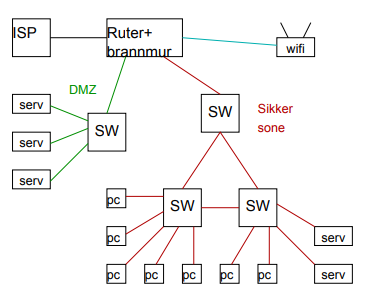
\includegraphics[scale=0.5]{firmanettverk.png}
\label{fig:firmanettverk}
\end{figure}
 Dette lar seg gjøre ved at hver kontorplass får ethernettutgang med en kabel lett tilgjengelig så kablet nett ikke er vanskeligere enn å koble til en mus. Deretter lokkes det med enorm oppgradering i hastighet(som de vil få av det kablete nettet). Dropbox byttes ut med en egenhostet Nextcloud slik at det nesten ikke merkes forskjell. Bob Kåre og alle annsatte blir kurset i det nødvendige i nye systemer og blir derettet overvåket og spurt regelmessig om det er noe i veien slik at de ikke går bak ryggen og lager hull. Om de er missfornøyd med noe kan dette forenkles på den rette måten. Serverrommet sikkres fra trivielle uhell med å vannsikre og muligens sette opp UPS.

 I tillegg settes det opp en backupserver som automatisk tar backup av det viktigste iløpet av natten, denne plaseres i et satelittkontor eller lignende, men her også sikkert og kryptert. Kviteringer og billag kan enkelt automatiseres og digitaliseres paralellt med enkle rutiner, disse backes også opp på backuptjeneren. I tillegg settes det inn sentral autentiseringsserver og en VPN de kan bruke for å få tilgang utenfor intærnnettet. Til sist av ting jeg kommer på i farten leies det ikke inn arbeidskraft for sensitivt arbeid. Dette er en trussel ledelsen ser ikke er nødvendig.


\subsection*{Sikkerhetspolicy}
Nettvett har en veldig fin veiledning her: \\ \url{https://nettvett.no/informasjonssikkerhetspolicy/}. \\Den skal i korte trekk utrykke ledelsens intensjoner og mål rundt informasjonssikkerhet slik at det er mulig å handle konsekvelt.

Først og fremst blir det kursing i trusselbildet for å sette en liten skrekk slik de ansatte følger med. Så konkrete handlinger de trenger å følge uten noen form for tvil. Adgangskort synlig, alltid koble til kablet nett, skjønne forskjellen på offentlig og privat filtjener, og påpeke at de skal si ifra om det er noe som helst de er missfornøyd med slik at det kan fikses på riktig måte.

\subsection*{Regler i brannmuren}
På grunn av tidspress har jeg ikke tid til å svare ordentlig på denne deloppgaven, håpen resten var utfyllende nok. Men en kort oversikt over type regler er å tilate bare porter vi tilbyr, blokkere pakker med opplagt forfalsket fra-address, umulige kombinasjoner av flagg, ugyldige fragmenter. Det burte også bli satt opp regler på utgående pakker skulle neon maskiner bli kompromitert.


\end{document}
